\begin{align*}
  &\text{Leon Fiethen 1728330}\\
 &\text{Janik Sperling 1728567}
.\end{align*}
\section*{Sheet 7}
Unclear if $u \in  \mathcal{C}(\mathbb{R}^{n} ) $ is $u : \mathbb{R}^{n} \to  \mathbb{R}$ or $u : \mathbb{R}^{n} \to \mathbb{R}^{n}  $, we consider the first case here
but it doesn't change any of the following proofs 
\subsection*{19. Twirling towards freedom}
Let $u \in  \mathcal{C}^{2}(\mathbb{R}^{n} ) $ be a harmonic function. Show that the following functions are also harmonic.\\[1ex]
\textbf{Note } Whenever we write $\frac{\partial v}{\partial x_i}$ we are really referring to $\tilde{x}(x)_i$  
\begin{exercise}[a]
  $v(x) = u(x+b) $ for $b \in  \mathbb{R}^{n} $ 
\end{exercise}
\begin{solution}
 Using chain rule gives 
 \begin{align*}
  \frac{\partial v}{\partial x_i}  = \frac{\partial u}{\partial x_i} *\frac{\partial (x+b)}{\partial x_i}  = \frac{\partial u}{\partial x_i }*1 
 .\end{align*}
 Second derivative gets another $* \ 1$. \\[1ex]
 Such that summing gives 
 \begin{align*}
  \triangle v =  1* \triangle u = 0
 .\end{align*}
\end{solution}
\begin{exercise}[b]
 $v(x) = u(ax)$  for $a \in  \mathbb{R}^{n} $
\end{exercise}
\begin{solution}
 Again using chain rule 
 \begin{align*}
  \frac{\partial v}{\partial x_i}  = \frac{\partial v}{\partial x_i} *\frac{\partial (ax)}{\partial x_i}  = \frac{\partial v}{\partial x_i }*a 
 .\end{align*}
 For the second derivative : 
 \begin{align*}
   \frac{\partial v}{\partial x_i}  = \frac{\partial^2 u}{\partial x_i^2} *\frac{\partial (ax)}{\partial x_i}*a  = \frac{\partial^2 u }{\partial x_i }*a^2
 .\end{align*}
 \begin{align*}
  \triangle v = a^2 \triangle u = a^2 * 0 = 0
 .\end{align*}
\end{solution}
\begin{exercise}[c]
 $v(x) = u(Rx)$ for $R(x_{1},\ldots,x_n) = (-x_{1},\ldots ,x_n)$ 
\end{exercise}
\begin{solution}
 Using chain rule
 \begin{align*}
   \frac{\partial v}{\partial x_i}  = \frac{\partial v}{\partial x_i} *\frac{\partial (Rx)}{\partial x_i}  = \begin{cases}
     -1 &\frac{\partial v}{\partial x_1} \text{ if } i=1\\
    &\frac{\partial v}{\partial x_i} 
   \end{cases}
 .\end{align*}
 Second derivative if $i=1$ we get another $-1$ and they cancel out s.t.
 \begin{align*}
   \frac{\partial ^2 v}{\partial x_i^2}  = \frac{\partial ^2 u}{\partial x_i^2} 
 .\end{align*}
 Summing gives 
 \begin{align*}
  \triangle v = \triangle u = 0
 .\end{align*}
\end{solution}
\begin{exercise}[d]
 $v(x) = u(Ax) $ for any orthogonal matrix $A \in  O(\mathbb{R}^{n} )$ 
\end{exercise}
\begin{solution}
  Note $(Ax)_i = \sum_{j=1}^{n} A_{ji}x_j $ such that using the chain rule 
\begin{align*} 
  \frac{\partial v}{\partial x_i}  = \frac{\partial u(Ax)}{\partial (Ax)_i}\frac{\partial Ax}{\partial x_i}  = \triangledown u *\underbrace{A_i}_{i\text{-th col}}
.\end{align*}
We get the gradient of $u$ since we take the derivative of $u$ with respect to $(Ax)_i$\\[1ex]
Second derivative 
\begin{align*}
  \frac{\partial}{\partial x_i} \frac{\partial v}{\partial x_i} =  \frac{\partial}{\partial (Ax)_i} \triangledown u(Ax) * A_i * \frac{\partial Ax}{\partial x_i}   = \triangledown * (\triangledown u*A_i)A_i 
.\end{align*}
Note since $A$ is orthogonal we get $A A^{T} = \cha $, writing out the terms as sum for clarity 
\begin{align*}
  \sum_{j,k = 1}^{n} \frac{\partial ^2 u}{\partial x_j \partial x_k} A_{ji}A_{ki}  = \sum_{i=1}^{n} \frac{\partial ^2 u }{\partial x_i^2}  = 0
.\end{align*}
\end{solution}
\newpage
\subsection*{20. Harmonic Polynomials in Two Variables}
\begin{exercise}[a]
 Let $u \in  \mathcal{C}^{\infty}(\mathbb{R}^{n} ) $ be a smooth harmonic function. Prove that any derivative of u is also harmonic
\end{exercise}
\begin{solution}
First note that $u^{(k)}(x_{0})  \in  \mathcal{C}^{\infty}(\mathbb{R}^{n} ) $ for any $k \in  \mathbb{N}$ \\ 
and $x_{0} \in  \mathbb{R}^{n} $ \\
\textbf{IA:} $k=1$
\begin{align*}
  \triangle (u^{(1)} ) = \begin{pmatrix} \frac{\partial ^2}{\partial x_i^2} , \ldots  , \frac{\partial ^2}{\partial x_i^2} \end{pmatrix}  \begin{pmatrix} \frac{\partial u(x_{0})}{\partial x_1} \\ \vdots \\ \frac{\partial u(x_{0})}{\partial x_n}\end{pmatrix}  = \sum_{i=1}^{n}  \frac{\partial ^2}{\partial x_i^2}* \frac{\partial u}{\partial x_i}  
.\end{align*}
The order of differentiation does not matter such that we get 
\begin{align*}
  \triangle (u^{(1)} ) = \frac{d}{dx} (\triangle u^{1} ) = 0
.\end{align*}
\textbf{IV:} Suppose the statement holds for $k \in  \mathbb{N}$ \\
\textbf{IS:} $k \to k+1$ \\
We know that $u^{(k)} \in \mathcal{C}^{\infty}(\mathbb{R}^{n} )  $ is harmonic by IV. such that by relabeling 
$u^{(k)}  \coloneqq  v \in \mathcal{C}^{\infty}(\mathbb{R}^{n} ) $ we can again apply the argument from the IA. which concludes the proof
\end{solution}
\begin{exercise}[b]
 Choose any positive degree n. Consider the complex valued function $f_n : \mathbb{R}^{2} \to  \mathbb{C}$ given by
$f_n(x, y) = (x+iy)^{n}$  and let $u_n(x, y)$ and $v_n(x, y)$ be its real and imaginary parts respectively.
Show that $u_n$ and $v_n$ are harmonic. 
\end{exercise}
\begin{solution}
  Treating the Laplacian in $\mathbb{C}$ as we do in $\mathbb{R}$ 
  \begin{align*}
    \partial_x f_n  &= n(x+iy)^{n-1} \\
    \partial_y f_n  &= n*i(x+iy)^{n-1} 
  .\end{align*}
  Then 
  \begin{align*}
    \triangle f_n &= n(n-1)(x+iy)^{n-2}  +(i^2n(n-1)(x+iy)) \\
    &= n(n-1)*\left( (x+iy)^{n-2} - (x+iy)^{n-2}   \right)  \\
    &= 0
  .\end{align*}
  Since $u_n,v_n$ are real and imaginary part , their Laplacian must be 0 as well.
  % We identify $\mathbb{C}$ with $\mathbb{R}^{2} $ by $ \phi  :\ \mathbb{R}^{2} \to  \mathbb{C} \ : \ (x,y) \mapsto x +iy$\\[1ex]
  % Then we consider $f_n = \phi \circ \tilde{f}_n$ where
  % \begin{align*}
  %   \tilde{f}_n \ : \ \mathbb{R}^{2}   \to  \mathbb{R}^{2}  \ (x,y) \mapsto \begin{pmatrix} u_n(x,y) \\ v_n(x,y) \end{pmatrix} 
  % .\end{align*}
  % Applying the Laplacian operator to   $\tilde{f}_n$ 
  % \begin{align*}
  %   \triangledown * (\triangledown \tilde{f}_n) =  \begin{pmatrix} \frac{\partial ^2 u}{\partial x^2}+ \frac{\partial ^2 u}{\partial y^2} , \frac{\partial ^2 v}{\partial x^2}+ \frac{\partial ^2 v}{\partial y^2}  \end{pmatrix} 
  % .\end{align*}
  % Now if we apply the chain rule to 
  % \begin{align*}
  %   \phi \circ \tilde{f}
  % .\end{align*}
  % Consider the Term 
  % \begin{align*}
  %   \frac{\partial \phi }{\partial \tilde{f}}  = (1,i)
  % .\end{align*}
  % And 
  % \begin{align*}
  %   \frac{\partial \phi }{\partial \tilde{f}}  = (1,i)
  % .\end{align*}
%   Using (a) and induction ($u_n$,$v_n$ harmonic) gives \\[1ex]
%   \textbf{IA} $n=1$ : 
%   \begin{align*}
%     f_1(x,y) = x+iy
%   .\end{align*}
%   Such that
%   \begin{align*}
%     u_1(x,y) = x \\
%     v_1(x,y) = y
%   .\end{align*}
%   Clearly $u$ and $v$ are twice differentiable (smooth even)  and 
%   \begin{align*}
%     \triangle u_1 &= 0 \\
%     \triangle v_1 &= 0
%   .\end{align*}
% \textbf{IV} suppose the statement holds for arbitrary  $n \in  \mathbb{N}$ \\
% \textbf{IS} $n\to n+1$ 
% We get 
% \begin{align*}
%   f_{n+1} = u_{n+1} + i*v_{n+1} 
% .\end{align*}
% Then consider 
% \begin{align*}
%   u_{n+1} = u_n + p(n)
% .\end{align*}
\end{solution}
\begin{exercise}[c]
 A  homogeneous polynomial of degree $n$ in two variables is a polynomial of the form 
 \begin{align*}
  p = \sum a_k x^{k}y^{n-k}  
 .\end{align*}
 Show that $\partial_x p$ and $\partial_y p$ are homogeneous of degree $n-1$
\end{exercise}
\begin{solution}
  Calculating 
  \begin{align*}
    \partial_x p = \frac{\partial}{\partial x} \sum_{k=0}^{n}  a_k x^{k} y^{n-k}   = \sum_{k=0}^{n} k*a_kx^{k-1}y^{n-k}  
  .\end{align*}
  For $k=0$ we have $ k*a_k = 0$ such that the first term vanishes
  \begin{align*}
    \sum_{k=0}^{n} k a_k x^{k-1}y^{n-k} = \sum_{k=1}^{n} k a_k x^{k-1}y^{n-k} = \sum_{i=0}^{n-1} (i+1)a_{i+1}x^{i}y^{(n-1)-i}   
  .\end{align*}
  For the case $\partial_y$ we get the term $(n-k)*a_k$ which is 0 for $k=n$  such that the last term of our sum vanishes 
  and the degree is reduced by 1 \\[1ex]
\end{solution}
\begin{exercise}[d]
 Show that such a homogeneous polynomial of degree n is harmonic if and only if it is a linear combination of $u_n$  and $v_n$
\end{exercise}
\begin{solution}
 "$\Leftarrow$":  Let $p$ be a linear combination of $u_n$ and $v_n$ then by (b) we know $u_n$ and $v_n$ are harmonic, since 
 the Laplacian is a linear operator, we conclude $p$ must also be harmonic. \\[1ex]
 Other direction is missing
\end{solution}
\subsection*{Louisville's Theorem}
Liouville’s theorem (3.9 in the script) says that if $u$ is bounded and harmonic, then $u$ is constant.
In this question we give a geometric proof in $\mathbb{R}^{2} $ using globular means defined when $B(x, r) \subset  \Omega $
through
\begin{align*}
  \mathcal{M}[v](x,r) = \frac{1}{\omega_nr^{n} } \int_{B(x,r)}v(y) dy
.\end{align*}
Recall from Theorem 3.5 that if u is harmonic then it obeys $u(x) = \mathcal{M}[u](x, r)$.
\begin{exercise}[a]
Consider two points $a,b$ in the plane which are distance $2d$ apart. Now consider two balls,
both with radius $r>d$, centered on the two points respectively. Show that the area of the intersection is 
\begin{align*}
  \text{area} B(a,r) \cap B(b,r) = 2r^2 a\cos(dr^{-1} ) - 2d\sqrt{r^2-d^2} 
.\end{align*}
\end{exercise}
\begin{solution}
  W.l.o.g we may assume $a = (0,0)$  and $b=(2d,0)$, otherwise we just shift the plane to be centered at a first and rotate (both volume preserving) \\[1ex]
  In that case we can solve for the points of intersection by 
  \begin{align*}
    x^2+y^2 = r^2 = (x-2d)^2 + y^2
  .\end{align*}
  Such that 
  \begin{align*}
    x^2 -(x-2d)^2 &= 0 \\
    x^2 -(x^2-4dx+4d^2) &= 0 \\
    4dx - 4d^2 &= 0 \\
    x = d
  .\end{align*}
  And y 
  \begin{align*}
    d^2 + y^2 = r^2 \implies y = \pm \sqrt{r^2-d^2} 
  .\end{align*}
  Now either by integrating we get 
  \begin{align*}
    x^2+y^2 = r^2 \implies x = \sqrt{r^2-y^2} 
  .\end{align*}
  \begin{align*}
    2*\left( \int_{-\sqrt{r^2-d^2} }^{\sqrt{r^2-d^2} } \sqrt{r^2-y^2}  dy - 2d*\sqrt{r^2-d^2}  \right) 
  .\end{align*}
  Or the prettier way \newpage
  \hspace{0mm}\\
  We can get the light-green area by calculating the area of the triangle and subtracting it from the area of the sector and multiplying by 4, this gives the following \\[1ex]
  Triangle area
  \begin{align*}
    \frac{1}{2} *d*\sqrt{r^2-d^2}  
  .\end{align*}
  Sector area , since $\theta = \cos^{-1}(\frac{d}{r})$ and the area of the sector is proportional to the angle where $\theta =2\pi $ 
  gives the full circle we get 
  \begin{align*}
    \frac{r^2 \theta }{2}
  .\end{align*}
  Putting it together 
  \begin{align*}
    &4*\left(\frac{r^2 \cos^{-1}(\frac{d}{r})}{2} -  \frac{d}{2}\sqrt{r^2-d^2} \right)\\
    &=2r^2\cos^{-1}(dr^{-1}) - 2d\sqrt{r^2-d^2} 
  .\end{align*}
  \begin{center}
    \begin{figure}[H] 
      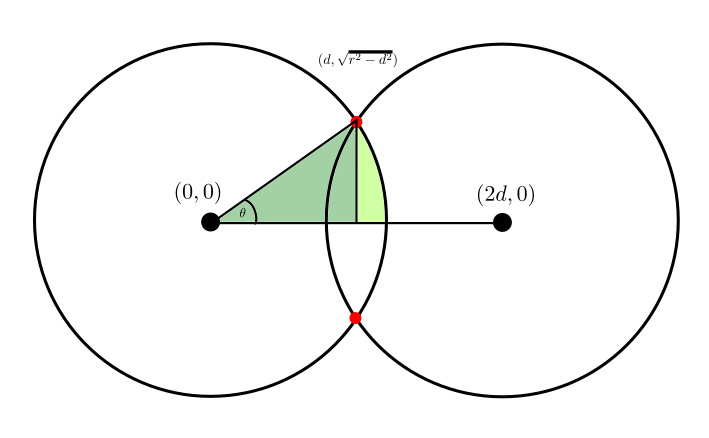
\includegraphics[scale=1]{figures/area_alternative.png}
   \end{figure} 
  \end{center}
\end{solution}
\newpage
\begin{exercise}[b]
 Suppose that $v$ is a bounded function on the plane $-C \le v(x) \le C$  for all x and some constant C. Show that 
 \begin{align*}
   \abs{\mathcal{M}[v](a,r) - \mathcal{M}[v](b,r)} \le \frac{2C}{\omega_2}(\pi -2a\cos(\frac{d}{r})) - \frac{2d}{r}\sqrt{1-d^2r^2} 
 .\end{align*}
\end{exercise}
\begin{solution}
  We get
  \begin{align*}
    \abs{\mathcal{M}[v](a,r) - \mathcal{M}[v](b,r)} &=\frac{1}{\omega_2r^{2} }  \abs*{\left(  \int_{B(a,r)} v(y) dy -  \int_{B(b,r)} v(y) dy \right)} \\
  .\end{align*}
  leaving the constant 
\begin{align*} 
  &=\abs*{\left(  \int_{B(a,r) \setminus B(b,r)} v(y) dy -  \int_{B(b,r) \setminus B(a,r)} v(y) dy \right)} \\
  &\le   \int_{B(a,r) \setminus B(b,r)} \abs*{v(y)} dy +  \int_{B(b,r) \setminus B(a,r)} \abs{v(y)} dy \\
  &\myS{def.}{\le } \int_{B(a,r) \setminus B(b,r)} C dy -  \int_{B(b,r) \setminus B(a,r)} C dy \\
.\end{align*}
Then by drawing a picture and looking at it we know 
\begin{align*}
  \text{area}(B(a,r) \setminus B(b,r)) + \text{area}(B(a,r) \setminus B(b,r)) =  2\pi r^2 - 2*\text{area}(B(a,r) \cap B(b,r))
.\end{align*}
Using (a)
\begin{align*}
  \abs{\mathcal{M}[v](a,r) - \mathcal{M}[v](b,r)} \le \frac{2C}{\omega_2}*\left(\pi - 2\cos^{-1}(\frac{d}{r})+\frac{2d}{r^2}\sqrt{r^2-d^2}  \right) 
.\end{align*}
\end{solution}
\begin{exercise}[c]
 Let $u \in  \mathcal{C}^{2}(\mathbb{R}^{2} ) $ be a bounded harmonic function. Complete the proof that u is constant 
\end{exercise}
\begin{solution}
 By Theorem 3.5 we know that
 \begin{align*}
   u(x) = \mathcal{M}[u](x,r)
 .\end{align*}
Picking any points $a,b \in  \mathbb{R}^{2} $ we check the distance
\begin{align*}
  \abs{u(a)-u(b)} = \abs{\mathcal{M}[u](a,r) - \mathcal{M}[u](b,r)} \le C(r,d)
.\end{align*}
Where $r >d \coloneqq  \|a-b\|$ , i.e 
\begin{align*}
  \lim_{h \to 0} \frac{\abs{u(a+h) - u(a)}}{h} &= \lim_{h \to 0} \frac{\abs{\mathcal{M}[u](a+h,r(h)) - \mathcal{M}[u](a,r(h))}}{h}\\
                                               &\le \lim_{h\to 0} \frac{1}{h} * C(r(h),h) \\
                                               &=0
.\end{align*}
Where $C(r(h),h) \to  0$ as $h\to 0$  , thus $u$ must be constant if it is bounded and harmonic
\end{solution}
\subsection*{Weak Tea}
In this question we try to generalise the idea of spherical means to distribution in the way 
suggested in the lectures. Let $\lambda_{\epsilon } : \mathbb{R} \to  \mathbb{R}$ be the standard mollifier and define a sphere mollifier 
\begin{align*}
  \Lambda_{x,r,\epsilon}(y) = \frac{\lambda_{\epsilon }(\abs{y-x}-r)}{n \omega_{n}\abs{y-x}^{n-1} }
.\end{align*}
\begin{exercise}[a]
  Describe the support of $\Lambda_{x,r,\epsilon }$ 
\end{exercise}
\begin{solution}
  By definition it is all $y$ such that $\Lambda_{x,r,\epsilon }(y) \neq 0$ i.e all y such that $\abs{y-x} - r \in \supp \lambda_{\epsilon} \coloneqq \overline{B(0,\epsilon)} $,
  Which gives
  \begin{align*}
    \abs{y-x} -r \le  \epsilon  \implies \abs{y-x} \le \epsilon + r
  .\end{align*}
  \begin{align*}
    y \in B(x,\epsilon +r)
  .\end{align*}
\end{solution}
\begin{exercise}[b]
  We may try to define the spherical mean of a distribution $F$ as $\lim_{\epsilon  \to  0} F(\Lambda_{x,r,\epsilon })$. However
this does not always exist. Let $G$ be the distribution in Exercise 17(d), submanifold inte-
gration on the unit circle. Show that $G(\Lambda_{0,1,\epsilon }) = \lambda_{\epsilon }(1)$ and therefore the limit does not
exist.
\end{exercise}
\begin{solution}
  First we can check that indeed  $\Lambda \in  \mathcal{C}^{\infty}_0 $ such that $G(\Lambda_{0,1,\epsilon })$ is valid 
 \begin{align*}
   \Lambda_{0,1,\epsilon } = \frac{\lambda_{\epsilon}(\abs{y}-1)}{2 \omega_2 \abs{y}}
 .\end{align*}
 We have $C \coloneqq  \{x^2+y^2 = 1\}  $ i.e $C \coloneqq  \partial B(0,1)$ then 
 \begin{align*}
   G(\Lambda_{0,1,\epsilon }) &= \int_{\{x^2+y^2=1\}  } \frac{\lambda_{\epsilon}(\abs{y}-1)}{2 \omega_2 \abs{y}} d\sigma\\
                              &= \int_{\partial B(0,1)}\frac{\lambda_{\epsilon}(0)}{2\omega_2} d\sigma  = \lambda_{\epsilon }(0)
 .\end{align*}
 If we didn't  shift by $r=1$ it would be 1. For $\epsilon  \to 0$ we have $\lambda_{\epsilon }(0) \to \infty$
\end{solution}
\begin{exercise}[c]
  Show that the limit $\lim_{\epsilon \to 0} F(\Lambda_{x,r,\epsilon })$ 
\end{exercise}
\begin{solution}
 Let $F$ be a harmonic distribution i.e $\triangle F = 0$ then  F has the weak mean value property by Theorem 3.6
 and we know that $F$ vanishes on any test function with $\int \psi d\mu = 0$ where $\psi \in  \mathcal{C}^{\infty}_0((0,r)) $\\
 We know that necessarily  we have 
\begin{align*}
 \int_\Omega  \Lambda_{x,r,\epsilon }  d\mu = 1 
.\end{align*} 
Choose any test function $\phi $ such that its integral is 1  then $\tilde{\phi } = \phi - \Lambda_{x,r,\epsilon}$  
\begin{align*}
  \int_\Omega  \tilde{\phi } = 0
.\end{align*}
Since distribution are linear operators 
\begin{align*}
  0 = F(\tilde{\phi }) = F(\phi) - F(\Lambda_{x,r,\epsilon })
.\end{align*}
Thus the limit exists.
\end{solution}
